\documentclass[a4paper,11pt]{article}

\usepackage[british]{babel}
\usepackage{indentfirst}
\usepackage{graphicx}
\usepackage{subcaption}
\usepackage{float}
\usepackage{chngcntr,tocloft}
\usepackage{listings}
\usepackage{comment}
\usepackage{fancyhdr}
\usepackage[utf8]{inputenc}
\usepackage{indentfirst}
\usepackage{amsmath}
\usepackage{textgreek}
\usepackage{fixltx2e}
\usepackage{color}
\graphicspath{ {images/} }
\usepackage{hyperref}
\hypersetup{
    colorlinks=false,
    linkcolor=blue,
    filecolor=magenta,      
    urlcolor=cyan,
    }
\definecolor{green}{rgb}{0,0.6,0}
\definecolor{gray}{rgb}{0.5,0.5,0.5}
\definecolor{mauve}{rgb}{0.58,0,0.82}

\lstset{ %
  backgroundcolor=\color{white},   
  basicstyle=\footnotesize,       
  breaklines=true,                 
  captionpos=b,                    
  commentstyle=\color{green},    
  escapeinside={\%*}{*)},          
  keywordstyle=\color{blue},       
  stringstyle=\color{mauve}, 
}


\counterwithin*{figure}{section}
\counterwithin*{figure}{subsection}
\counterwithin*{figure}{subsubsection}

\addtolength{\cftfignumwidth}{2em}

\renewcommand{\thefigure}{%
  \ifnum\value{subsection}=0
    \thesection.\arabic{figure}%
  \else
    \ifnum\value{subsubsection}=0
      \thesubsection.\arabic{figure}%
    \else
      \thesubsubsection.\arabic{figure}%
    \fi
  \fi
}

\begin{document}

\begin{titlepage}
	\centering
	{\scshape\LARGE Warsaw University of Technology \par}
	\vspace{1cm}
	{\scshape\Large Faculty of Power and Aeronautical Engineering\par}
	\vspace{5cm}
	{\huge\bfseries Modelling the Von Karman vortex path using OpenFOAM 8\par}
	\vspace{5cm}
	{\Large\ Kamil Kozłowski\par}
	\vfill
	Computer Simulations of Combustion Processes\par
	\vfill

% Bottom of the page
	{\large June 2021\par}
\end{titlepage}

\tableofcontents
\newpage



\section{Introduction}
  
 
\begin{figure}[h]
\centering
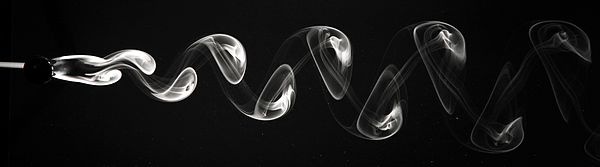
\includegraphics[width=12cm]{vortecies.JPG}
\caption{von Karman vortecies}
\end{figure}

This report is devoted to numerical modelling of the von Karman vortex path. This phenomenon is about generating vortices on an obstacle placed perpendicular to the flowing medium (liquid or gas). It is an object of observations for hundreds of years, as evidenced by example sketches showing vortices forming on
river drawn by Leonardo da Vinci himself. \par			Feature a characteristic of the phenomenon is that vortices arise alternating once on one side of the obstacle and the frequency of their generation is directly proportional to stream velocity. This property was discovered in 1878 by Strouhal by observing the change in the pitch of the generated sounds on the wire exposed to the wind. He came to
the conclusion that the pitch increases with a growth of a wind speed and decreases with an increasing wire diameter. A year later, in 1879, Lord Rayleigh discovered that the phenomenon of vortex forming is accompanied perpendicular to the stream
lifting force.\par
	An essential step in the development of fluid mechanics
was to define in 1883 by O. Reynolds
conditions under which laminar flow becomes
turbulent. Based on observations of the water flow in a glass tube to which the dye was brought, a dimensionless criterion number has been defined
to estimate the flow stability. This number,
later named the Reynolds number, is the ratio of the forces of inertia to the forces of viscosity and is expressed as follows:
\begin{gather*}
    Re = \frac{vd}{\nu}
\end{gather*}

\noindent where: v - the free stream flow speed,  d - a characteristic length parameter of the body or channel, \textnu \ - the free stream kinematic viscosity parameter

\medskip
 
A milestone in research on understanding
the phenomenon of vortex generation was published in 1911 the study of von Karman. He made the conclusion that the vortex generation does
regular character and the frequency of their occurrence gives write the equation:
\begin{gather*}
    f = S_T\frac{v}{d}
\end{gather*}

\noindent where: S\textsubscript{T}\ - Strouhal number

\medskip
 
A very important value of the phenomenon is the fact that the frequency of the vortexes generated in the obstacle does not depends on the physical properties, and only on its analysis speed. The result of the measurement does not depend on parameters such as temperature or chemical composition.\par
The results show unequivocally that the Strouhal number is invariant in a very wide range of Reynolds numbers. Very clearly it can be seen in the diagram shown in Fig. 2.1, taken from the publication of Yamasaki and Rubin in 1974.

\begin{figure}[h]
\centering
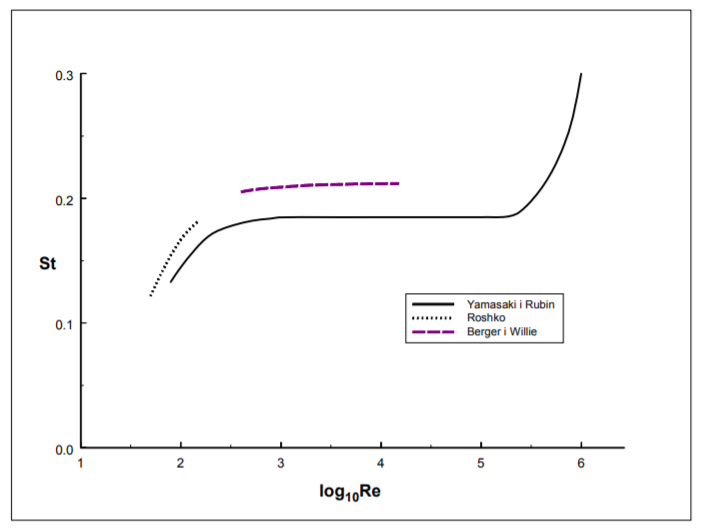
\includegraphics[width=10cm]{strouhal.PNG}
\caption{The dependence of the Reynolds number on the Strouhal number}
\end{figure}

For the range of numbers Re investigated by Berger and Willie changes are very slight. It does
precisely the linearity of the frequency characteristic generated vortices as a function of flow velocity.

\section{Numerical modelling}

Navier-Stokes equation in vector form is as follows:
\begin{gather*}
    \frac{dv}{dt} = F - \frac{1}{\rho}grad(p)+\nu\nabla^2v+\frac{\nu}{3}grad(div(v))
\end{gather*} 
\noindent where: F - mass force vector.
\medskip
Taking into account the continuity equation:
\begin{gather*}
    \frac{dp}{dt} + \rho div(v) = 0
\end{gather*}
and the fact that for incompressible fluid ($\rho=0$):
\begin{gather*}
    div(v) = 0
\end{gather*}
we obtain general flow equation for the incompressible
Newtonian fluid:
\begin{gather*}
    \frac{dv}{dt} = F - \frac{1}{\rho}grad(p)+\nu\nabla^2v
\end{gather*}

\noindent This equation can be solved by numerical methods. The DNS method gives the best results, as a result of which a full instantaneous velocity field of the analysed flow is obtained.

\section{Implementating the task in OpenFOAM-v2012}
	
	OpenFOAM (for "Open-source Field Operation And Manipulation") is a C++ toolbox for the development of customized numerical solvers, and pre-/post-processing utilities for the solution of continuum mechanics problems, most prominently including computational fluid dynamics (CFD).
	
\subsection{Creating a channel's geometry}

\begin{figure}[h]
\centering
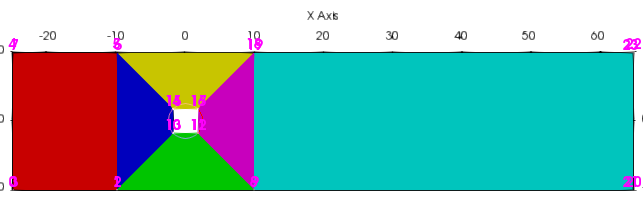
\includegraphics[width=11cm]{geometry.PNG}
\caption{Channel's geometry}
\end{figure}\par

The geometry was divided into 6 simple figures. The channel's width has been set to 20 cm and the length to 90 cm. The geometry is in 2D space, in this way channel's length on the z coordinate has to be equal one. In 3D space, the upper surface of the channel has z coordinate equal to constant +0.5 and the lower to -0.5. These 6 blocks were created in  \emph{blockMeshDict} file in \emph{systems} by giving vertex coordinates of each block in 3D space.

The beginning of the adopted global coordinate system is at obstacle's centre point. The obstacle is a cylinder with a diameter of 5 cm.	

\subsection{Preparing a mesh}

\begin{figure}[h]
\centering
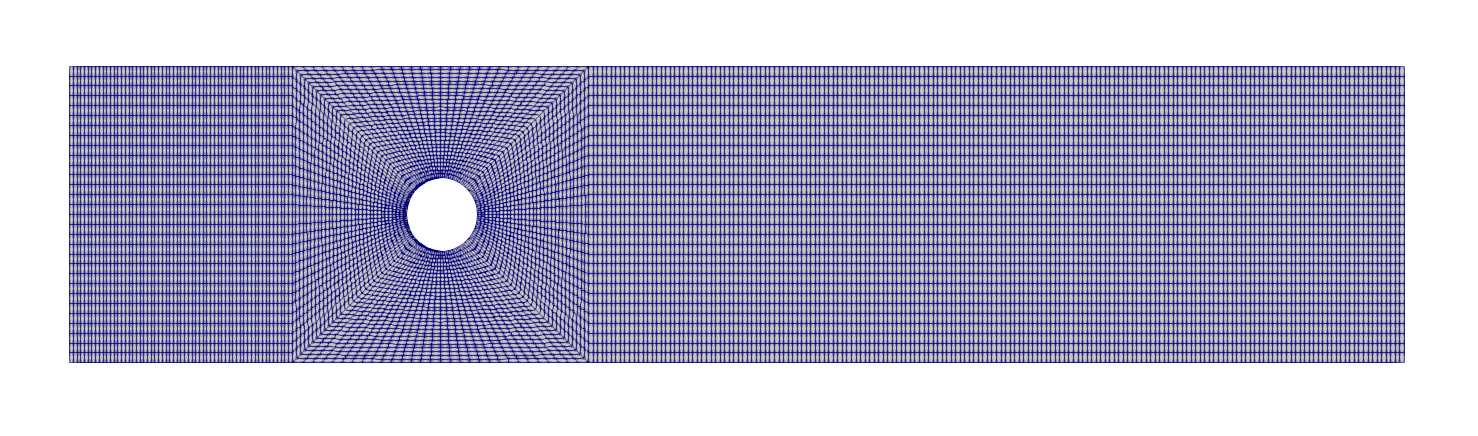
\includegraphics[width=14cm]{mesh.PNG}
\caption{Mesh}
\end{figure}

The mesh consists of rectangles. A square part with the obstacle in it, has been sized into 30 divisions. Additionally, the mesh is fined close to cylinder's face, which affects the reliability of results. In this simple simulation refining the mesh at the boundary layer has been omitted. The elements of mesh are located in \emph{polyMesh} in \emph{constant} catalogue.
	
\subsection{Boundary conditions and solver settings}

Boundary conditions are set in \emph{0} folder. There are two files \emph{P} and \emph{U} which enables us to set initial pressure and velocity. In this simulation we do not impose any inlet pressure .

In case of velocity, the magnitude is calculated from the Reynolds number which in this study is equal to $Re = 1800$. Respecting characteristic length parameter which is equal to cylinder diameter $d=0.05 $ m and the free stream kinematic viscosity for water equal to $\nu=1,5\cdot10^{-5}\frac{m^{2}}{s}$, the fluid velocity is as follows:

\begin{gather*}
    v = \frac{Re\cdot\nu}{d} = 0.54 \frac{m}{s}
\end{gather*}

Turbulence model is set in the \emph{turbulenceProperties} in a folder named \emph{constant}. The Reynolds number equals 1800 is less than 2300 so we assume a laminar model of turbulence.
		
A solver could be choose in \emph{controlDict} file in \emph{systems}. For this kind of simulations solver called \emph{SimpleFoam} is appropriate. Writing interval is set to 100 steps and the calculations end at 10000 iterations.

\newpage

\section{Calculations}

Calculation required a few minutes. After this time, we saw that the results had beed written to the main folder. In the terminal we can type \emph{paraFoam} to visualize them (I was using ParaView 5.6.0). After reading the \emph{controlDict} file we click apply and the visualizations are ready.

The contours of velocity magnitude are presented below: 

\begin{figure}[h]
\centering
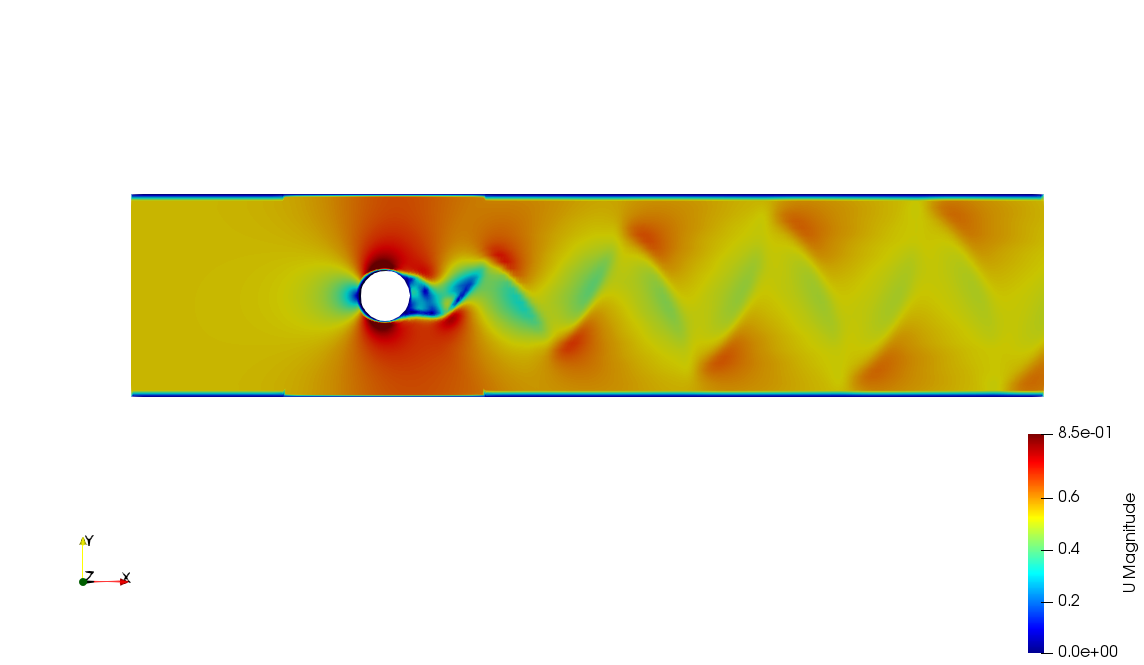
\includegraphics[width=14cm]{velocity.PNG}
\caption{Velocity magnitude contours}
\end{figure}

We observe that around the cylinder the flow accelerates and the maximum magnitude equals $0.85\frac{m}{s}$. In front of it there is a point of stagnation where the velocity is very low. Behind the cylinder we can see recirculation vortices which are presented in blue colour. In the further part of the channel we observe characteristic von Karman vortices, similar to these presented on the fig. 1.1. In my repository, an animation of this simulation has been uploaded.

\newpage

On the figure below we see contours of static pressure:

\begin{figure}[h]
\centering
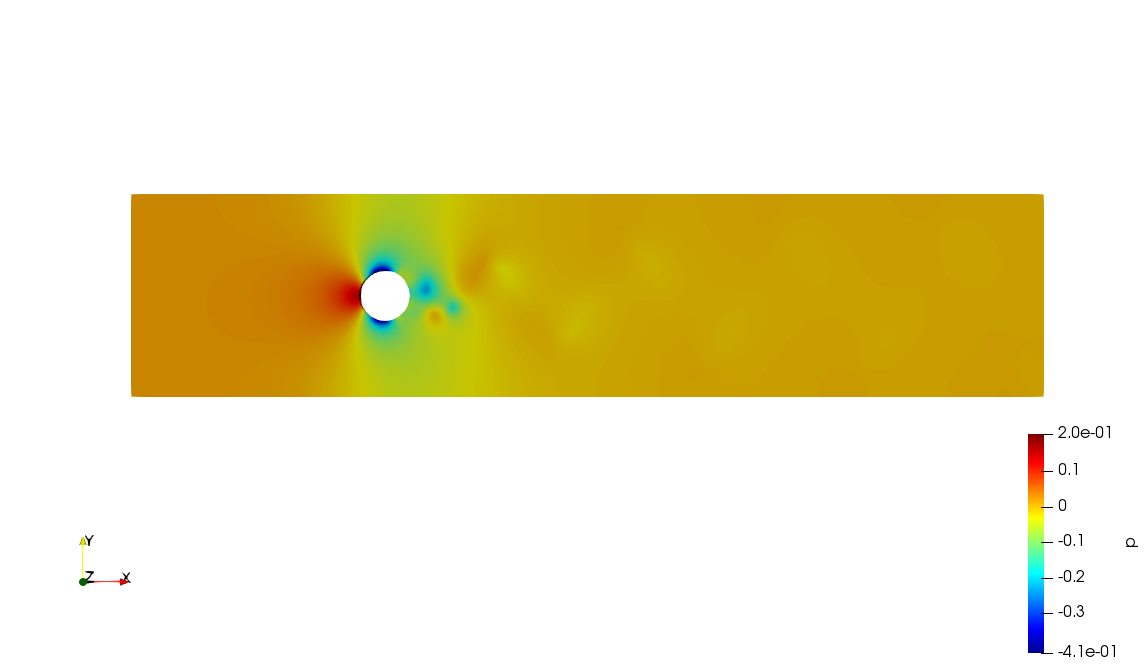
\includegraphics[width=14cm]{pressure.PNG}
\caption{Static pressure contours}
\end{figure}

According to the Bernoulli’s law, where the flow's velocity increases, the static pressure drops. The greatest magnitude is visible in front of the cylinder, where the water pushes on it.

\section{Conclusion}

\emph{OpenFoam} is an open source software enabling us to solve plenty of problems in the field of physics, especially fluid mechanics. It's most valuables advantages are:

\begin{itemize}
  \item free access
  \item being upgraded by users from all around the World
  \item a possibility to visualize results in GUI - ParaView 
  \item availability of repositories and tutorials 
\end{itemize}

Von Karman vortices are interesting phenomenon in fluid mechanics. In nature they appear as spiralling cloud patterns in the sky. They arise when winds are diverted around a blunt, high-profile area, often an island rising from the ocean. The alternating direction of rotation in the air forms swirls in the clouds.

\begin{figure}[h]
\centering
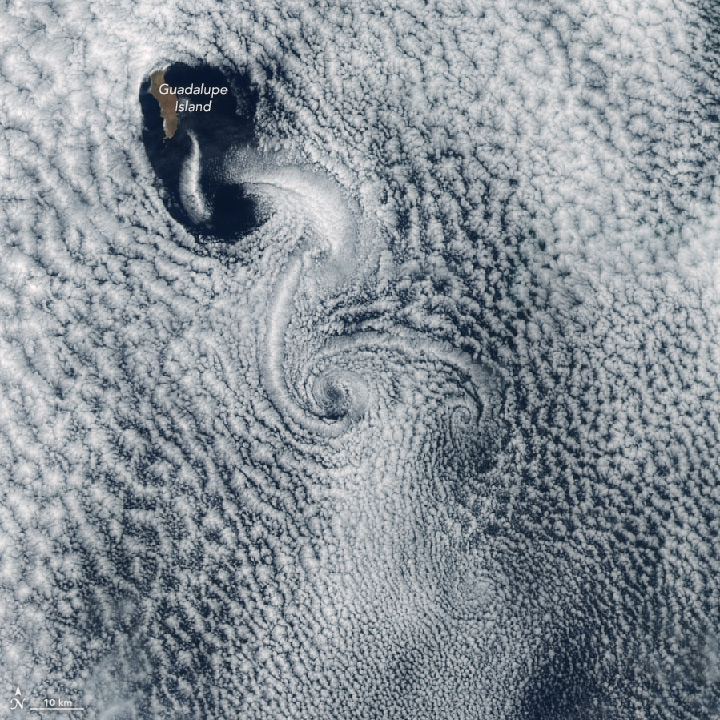
\includegraphics[width=6cm]{guadalupe.JPG}
\caption{Guadalupe Island, May 2017}
\end{figure}

\newpage

Satellites regularly spot these wind and cloud patterns around the world. On May 24, 2017, the Visible Infrared Imaging Radiometer Suite (VIIRS) on the Suomi NPP satellite captured a natural-colour image of such swirls on the lee side of Guadalupe Island. The volcanic island rises from the Pacific Ocean off the coast of Baja California, Mexico.

\begin{figure}[h]
\centering
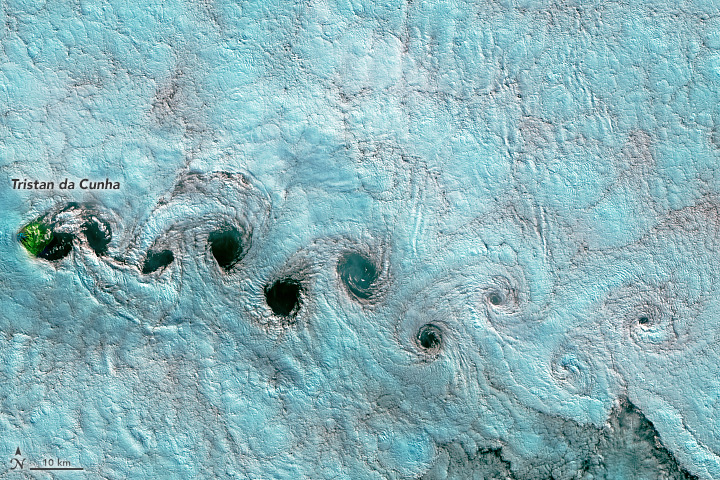
\includegraphics[width=8cm]{tristan.JPG}
\caption{Tristan da Cunha, June 2017}
\end{figure}

The second image shows the same phenomenon occurring an ocean basin away, on the lee side of Tristan da Cunha — a remote volcanic island in the South Atlantic. The image was captured on June 25, 2017, by the Operational Land Imager (OLI) on the Landsat 8 satellite. The image is false-colour (OLI bands 6-5-3) to better distinguish areas of land, water, and clouds.


\section{References}
 
\begin{enumerate}

\item  Artur KULIŃCZAK, Grzegorz PANKANIN, \textit{Modelowanie ścieżki wirowej von Karmana przy użyciu pakietu
ANSYS FLUENT} 2014
\\*
\url{http://pe.org.pl/articles/2014/8/46.pdf}

\item  Asmaa Hadane, \textit{How to simulate a Flow around Cylinder - Von Karman in OpenFoam} 28 Mai 2020\\*
\url{https://www.youtube.com/watch?v=YfK53PKpdgE&t=151s}

\item  Asmaa Hadane, \textit{OpenFOAM Tutorial: Simulation of the flow around a cylinder} 1 February 2021\\*
\url{https://www.youtube.com/watch?v=Udt3RhkbgKw}

\item \url{https://github.com/AsmaaHADANE/Youtube-Tutorials.git}

\item \url{https://en.wikipedia.org/wiki/K%C3%A1rm%C3%A1n_vortex_street#:~:text=In%20fluid%20dynamics%2C%20a%20K%C3%A1rm%C3%A1n,a%20fluid%20around%20blunt%20bodies.}

\item \url{https://earthobservatory.nasa.gov/images/90734/two-views-of-von-karman-vortices#:~:text=These%20so%2Dcalled%20%E2%80%9Cvon%20K%C3%A1rm%C3%A1n,cloud%20patterns%20around%20the%20world.}

\end{enumerate}

\end{document}
